\documentclass[tikz,border=10pt]{standalone}
\usepackage{tikz}
\usetikzlibrary{calc}

\begin{document}
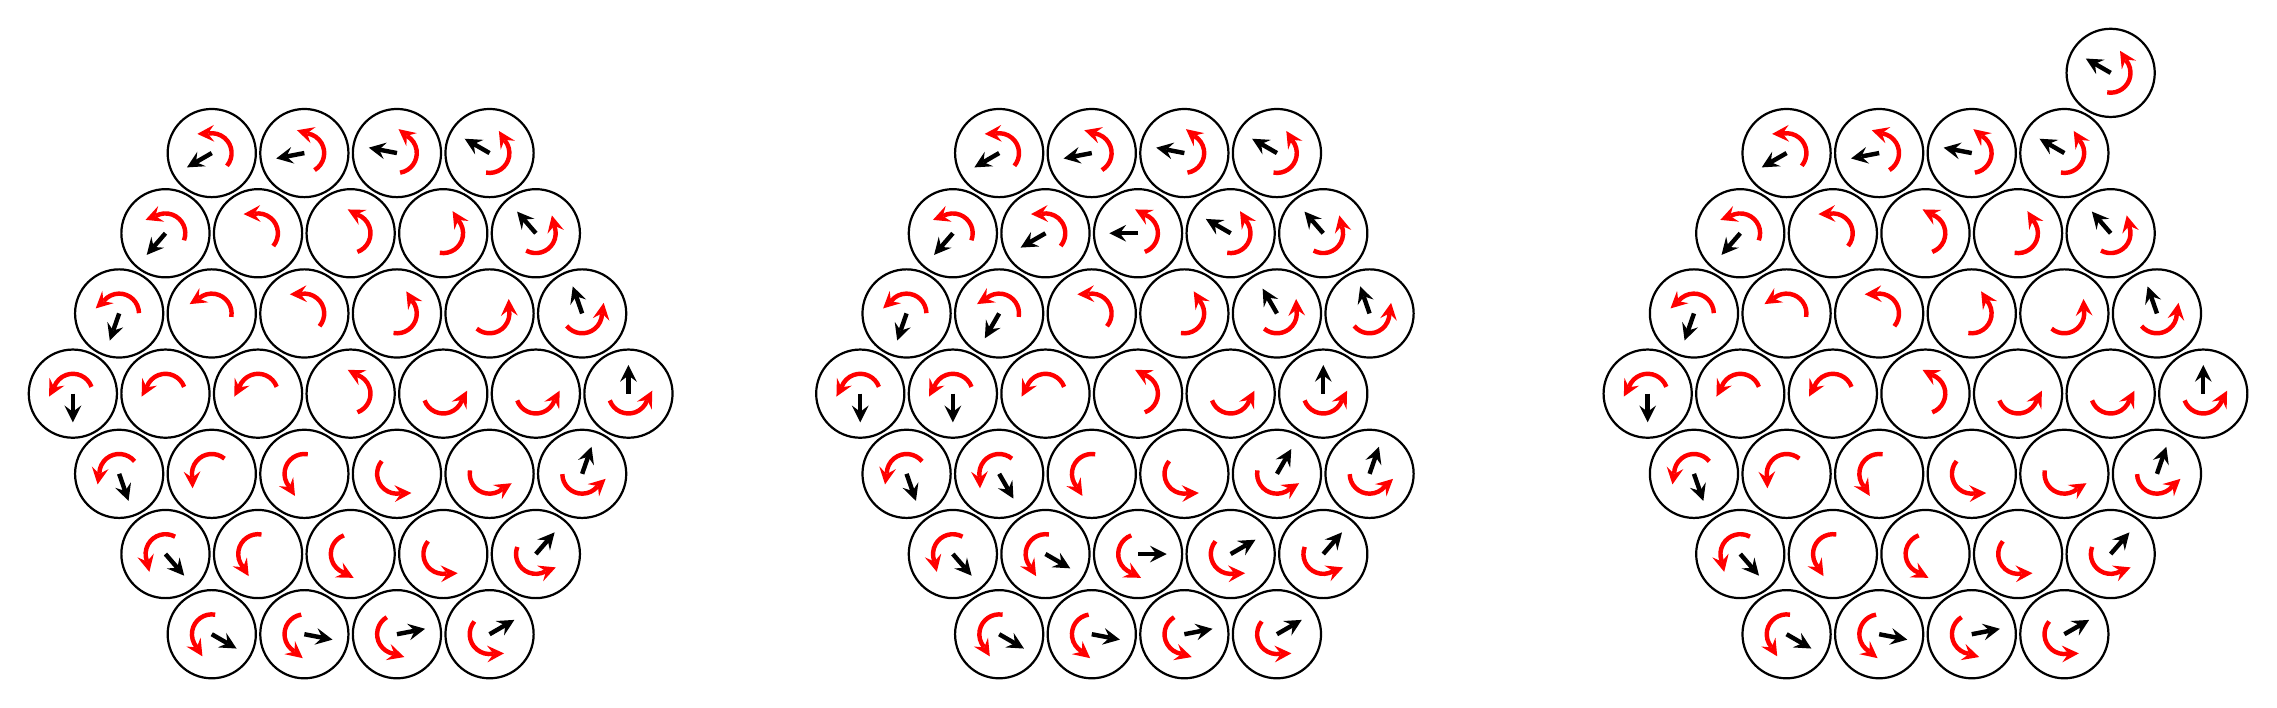
\begin{tikzpicture}[scale=2, >=stealth] % straight triangular arrowheads

% -----------------------
% PARAMETERS
% -----------------------
\def\sphereR{0.28}                     % circle radius
\pgfmathsetmacro{\gapFactor}{1.05}     % spacing factor to avoid overlap
\pgfmathsetmacro{\ringSpacing}{2*\sphereR*\gapFactor}
\pgfmathsetmacro{\sqrtThreeOverTwo}{0.86602540378}

% Arrow styling
\def\arrowLineWidth{1.6pt}            % arrow line width (doubled)
\def\blackArrowLenFactor{0.65}        % black arrow length factor (relative to sphereR)
\def\redArcRadiusFactor{0.45}         % red arc radius factor (relative to sphereR)
\def\redArcHalfSpan{70}               % half angular span (degrees) for red arc
\def\redTipOffset{8}                  % rotate red arrowhead clockwise by this many degrees
\pgfmathsetmacro{\redHeadLen}{\sphereR*0.25} % length of the short red arrowhead segment

% Layout
\pgfmathsetmacro{\subfigSep}{5.0}     % horizontal separation between subfigure centers
% Move crystals down by about two full circles (two diameters = 4*sphereR)
\pgfmathsetmacro{\downshift}{-4*\sphereR}

% -----------------------
% draw a single sphere (circle) at numeric coordinates (x,y)
% with the two arrows as specified
% #1 = x, #2 = y, #3 = drawBlack (1 or 0)
% -----------------------
\newcommand{\drawsphere}[3]{%
  \begin{scope}[shift={({#1},{#2})}]
    % circle (sphere)
    \draw[thick] (0,0) circle (\sphereR);

    % compute the black arrow angle: tangent direction = atan2(y,x)+90
    \pgfmathsetmacro{\ang}{atan2(#2,#1)+90}%

    % draw black arrow only if #3==1
    \ifnum#3=1
      % draw black arrow shorter so it ends inside the circle (leaving margin)
      \pgfmathsetmacro{\blacklen}{\sphereR*\blackArrowLenFactor}
      \draw[line width=\arrowLineWidth,->] (0,0) -- (\ang:\blacklen);
    \fi

    % compute red arc angles so the arc is centered opposite the black arrow
    \pgfmathsetmacro{\opposite}{\ang+180}%
    \pgfmathsetmacro{\startang}{\opposite - \redArcHalfSpan}%
    \pgfmathsetmacro{\endang}{\opposite + \redArcHalfSpan}%

    % red arc (drawn without an arrow tip)
    \pgfmathsetmacro{\redrad}{\sphereR*\redArcRadiusFactor}
    \draw[line width=\arrowLineWidth,red] (\startang:\redrad) arc[start angle=\startang, end angle=\endang, radius=\redrad];

    % place a straight arrowhead at the end of the red arc:
    % compute arrow direction: tangent at arc end is endang+90; rotate clockwise by redTipOffset
    \pgfmathsetmacro{\arrowDir}{\endang + 90 - \redTipOffset}
    \draw[line width=\arrowLineWidth,red,->] (\endang:\redrad) -- ++(\arrowDir:\redHeadLen);

  \end{scope}%
}

% -----------------------
% Helper: draw hex cluster up to ring R using axial coords (q,r)
% This uses the cube-distance test max(|q|,|r|,|s|) <= R
% The macro uses \removeBlackUpTo (integer) to decide whether to draw black arrows:
%   if dist <= \removeBlackUpTo  -> do NOT draw black arrow (pass 0)
%   else                           -> draw black arrow (pass 1)
% It also respects global \skipQ and \skipR to omit a single sphere (for the 18-sphere case).
% -----------------------
\newcommand{\drawClusterUpToR}[1]{%
  % #1 = R (integer)
  \pgfmathtruncatemacro{\Rval}{#1}
  \foreach \q in {\numexpr -\Rval\relax,...,\Rval}{
    \foreach \r in {\numexpr -\Rval\relax,...,\Rval}{
      \pgfmathsetmacro{\s}{-(\q)-(\r)}
      \pgfmathsetmacro{\dist}{max(abs(\q),abs(\r),abs(\s))}
      \pgfmathtruncatemacro{\disti}{\dist}
      \ifnum\disti>\Rval
        % outside cluster: do nothing
      \else
        % check skip coordinates
        \pgfmathtruncatemacro{\isSkip}{0}
        \ifnum\q=\skipQ
          \ifnum\r=\skipR
            \pgfmathtruncatemacro{\isSkip}{1}
          \fi
        \fi
        \ifnum\isSkip=0
          % decide whether to draw black arrow based on \removeBlackUpTo
          \pgfmathtruncatemacro{\drawBlackFlag}{0}
          \ifnum\disti>\removeBlackUpTo
            \pgfmathtruncatemacro{\drawBlackFlag}{1}
          \fi
          % axial -> cartesian coordinates for hex lattice
          \pgfmathsetmacro{\x}{\ringSpacing*(\q + 0.5*(\r))}
          \pgfmathsetmacro{\y}{\ringSpacing*(\sqrtThreeOverTwo*(\r))}
          \drawsphere{\x}{\y}{\drawBlackFlag}
        \fi
      \fi
    }
  }
}

% -----------------------
% Default skip coordinates: none (set to impossible values)
% -----------------------
\pgfmathtruncatemacro{\skipQ}{999}
\pgfmathtruncatemacro{\skipR}{999}

% -----------------------
% CONFIGURATION 1 (left): remove black arrows for rings 0..2 (center + next two rings)
% left cluster is full (19 spheres) so no skip
% -----------------------
\begin{scope}[shift={(-\subfigSep,{\downshift})}]
  \pgfmathtruncatemacro{\removeBlackUpTo}{2} % remove black arrows for dist <= 2
  \pgfmathtruncatemacro{\skipQ}{999}         % no skip
  \pgfmathtruncatemacro{\skipR}{999}
  \drawClusterUpToR{3}
\end{scope}

% -----------------------
% CONFIGURATION 2 (center): remove black arrows for rings 0..1 (center + next ring)
% center cluster should be missing one sphere (18 spheres) -> skip axial (3,0)
% -----------------------
\begin{scope}[shift={(0,{\downshift})}]
  \pgfmathtruncatemacro{\removeBlackUpTo}{1} % remove black arrows for dist <= 1
  \pgfmathtruncatemacro{\skipQ}{3}           % skip the sphere at axial (3,0)
  \pgfmathtruncatemacro{\skipR}{0}
  \drawClusterUpToR{3}
\end{scope}

% -----------------------
% CONFIGURATION 3 (right): remove black arrows for rings 0..2 (center + next two rings)
% right cluster is full (19 spheres) so no skip
% -----------------------
\begin{scope}[shift={(\subfigSep,{\downshift})}]
  \pgfmathtruncatemacro{\removeBlackUpTo}{2} % remove black arrows for dist <= 2
  \pgfmathtruncatemacro{\skipQ}{999}         % no skip
  \pgfmathtruncatemacro{\skipR}{999}
  \drawClusterUpToR{3}
  % add one extra at axial (q=0,r=4) with same black-arrow rule
  \pgfmathsetmacro{\xextra}{\ringSpacing*(0 + 0.5*(4))}
  \pgfmathsetmacro{\yextra}{\ringSpacing*(\sqrtThreeOverTwo*(4))}
  % extra has dist=4 so it will get a black arrow (dist>removeBlackUpTo)
  \drawsphere{\xextra}{\yextra}{1}
\end{scope}

\end{tikzpicture}
\end{document}